\documentclass[11pt, titlepage]{article}
\author{Caleb Logemann}
\title{MATH 666: Finite Element Methods \\ Homework 3}
\date{December 4, 2018}
\usepackage[letterpaper, margin=2cm]{geometry}
\usepackage{MATH666}
\usepackage{booktabs}
\usepackage{tikz}
\usetikzlibrary{shapes.geometric}
\usetikzlibrary{arrows}

\begin{document}
\maketitle

%\lstinputlisting[language=MATLAB]{H01_23.m}
\begin{enumerate}
  \item[\#1]
    Consider the Crank-Nicolson-cG(1) FEM for the diffusion equation.
    Find $u^n_h \in V^1_h$ such that
    \begin{gather*}
      \abr{\frac{u^n_h - u^{n-1}_h}{\delta t}, v} +
      \abr{\nabla \p{\frac{u^n_h + u^{n-1}_h}{2}}, v} = 
      \abr{\frac{f^n + f^{n-1}}{2}, \nabla v}
      \quad \forall v \in V^1_h, \quad \forall n = 1, 2, 3, \ldots \\
      \abr{u^0_h, v} = \abr{u_0, v}.
    \end{gather*}
    Following the convergence proof of the Backward-Euler-cG(1) FEM from class,
    prove that the Crank-Nicolson-cG(1) FEM satisfies:
    \[
      \norm{u^n_h - u(t^n)} = \mcO\p{\Delta t^2 + h^2}
    \]

    \begin{proof}
      The initial variational problem is formulated as finding $u \in V$ such that
      \begin{gather*}
        \abr{u_t, v} + \abr{\grad u, \grad v} = \abr{f, v} \quad \forall v \in V \\
        \abr{u(0, x), v} = \abr{u_0, v}
      \end{gather*}
      The semidescrete form of the FEM can be expressed as finding $u_h \in V^1_h$
      such that
      \[
        \abr{\p{u_h}_t, v} + \abr{\grad u_h, \grad v} = \abr{f, v} \quad \forall v \in V^1_h
        \abr{u_h(0, x), v} = \abr{u_0, v}
      \]

      I will also make use of the following projection $R_h(u)$ which satisfies
      \[
        \abr{\grad R_h(u), \grad v} = \abr{\grad u, \grad v} \quad \forall v \in V^1_h
      \]

      Suppose $u$ is the solution to the original variational problem, then
      for all $v \in V^1_h$,
      \begin{align*}
        \abr{u_t, v} + \abr{\grad u, \grad v} &= \abr{f, v} \\
        \abr{u_t, v} + \abr{\grad R_h(u), \grad v} &= \abr{f, v} \\
      \end{align*}
      This is true for every time $t > 0$, in particular it is true at times
      $t^n$ and $t^{n-1}$, so
      \begin{align*}
        \abr{u^n_t, v} + \abr{\grad R_h(u^n), \grad v} &= \abr{f^n, v} \\
        \abr{u^{n-1}_t, v} + \abr{\grad R_h(u^{n-1}), \grad v} &= \abr{f^{n-1}, v} \\
        \abr{\frac{u^n_t + u^{n-1}_t}{2}, v} + \abr{\grad R_h\p{\frac{u^n + u^{n-1}}{2}}, \grad v} &= \abr{\frac{f^n + f^{n-1}}{2}, v} \\
        \abr{\grad R_h\p{\frac{u^n + u^{n-1}}{2}}, \grad v} &= \abr{\frac{f^n + f^{n-1}}{2}, v} - \abr{\frac{u^n_t + u^{n-1}_t}{2}, v}\\
      \end{align*}
      Consider $u^n_h$ and $u^{n-1}_h$, solutions to the FEM, they satisfy
      \[
        \abr{\frac{u^n_h - u^n_h}{\delta T}, v} + 
        \abr{\grad \frac{u_h^n + u_h^{n-1}}{2}, \grad v} = 
        \abr{\frac{f^n + f^{n-1}}{2}, v} 
      \]
      Let $\theta^n = R_h u^n - u^n_h$, then subtracting the last two equations
      gives
      \begin{align*}
        test
      \end{align*}
      
    \end{proof}

  \item[\#2] % Done
    Consider the non-conforming FEM for the Poisson equation using the linear
    Crouzeix-Raviart element discussed in class:
    \begin{enumerate}
      \item[(a)] % Done
        Explicitly write out the stiffness matrix on a uniform Cartisian mesh
        (with triangles created by cutting each Cartesian square into two
        triangles) on $\br{0,1} \times \br{0, 1}$.

        First I will define some notation.
        For the Cartesian mesh, let $M$ be the number of interior nodes along
        one axis, then $h = \frac{1}{M+1}$.
        Now the coordinates of the nodes of the Cartesian mesh will be
        $x_i = ih$ and $y_j = jh$, for $i, j = 0, \ldots, M+1$.
        We can also denote the midpoints as $x_{i+1/2} = ih + \frac{h}{2}$ and $y_{j+1/2} = jh + \frac{h}{2}$.
        For the Crouzeix-Raviart element, the midpoints of the edges of the
        triangles are the important points.
        These points will be at $(x_{i+1/2}, y_{j+1/2})$ for $i, j = 0, \ldots, M$,
        $(x_i, y_{j+1/2})$ for $i = 1, \ldots, M$ and $j = 0, \ldots, M$, and at
        $(x_{i+1/2}, y_{j})$ for $j = 1, \ldots, M$ and $i = 0, \ldots, M$.
        Below is the image of how one cell in the Cartesian mesh is transformed
        into two Crouzeix-Raviart elements.
        The image also describes some notation that I will use.
        The lower left triangle/region, I will label $\mbT^{(i, j)}_1$ and the upper
        right triangle will be $\mbT^{(i, j)}_2$.
        The basis functions for each node are labeled as described.

        \tikzstyle{vertex_style}=[circle, draw, inner sep=2pt, align=center]
        \tikzstyle{dot_style}=[circle, draw, fill=black, radius=1pt,inner sep=1.5pt]
        \begin{center}
          \begin{tikzpicture}
            \coordinate[](a) at (0, 0) {};
            \node[] at (0, -.3) {$x_{i}$};
            \node[dot_style](b) at (2, 0) {};
            \node[align=right] at (2, .4) {$\phi^{(i, j)}_{1}$};
            \node[] at (2, -.3) {$x_{i+1/2}$};
            \coordinate[](c) at (4, 0) {};
            \node[] at (4, -.3) {$x_{i+1}$};
            \node[align=right] at (4.5, 0) {$y_{j}$};
            \node[dot_style](d) at (0, 2) {};
            \node[align=right] at (.5, 2) {$\phi^{(i, j)}_2$};
            \node[dot_style](e) at (2, 2) {};
            \node[align=right] at (1.6, 1.7) {$\phi^{(i, j)}_{hyp}$};
            \node[dot_style](f) at (4, 2) {};
            \node[align=right] at (3.3, 2) {$\phi^{(i+1, j)}_{2}$};
            \node[align=right] at (4.7, 2) {$y_{j+1/2}$};
            \coordinate[](g) at (0, 4) {};
            \node[dot_style](h) at (2, 4) {};
            \node[align=right] at (2, 3.6) {$\phi^{(i, j+1)}_{1}$};
            \coordinate[](i) at (4, 4) {};
            \node[align=right] at (4.5, 4) {$y_{j+1}$};
            \node[align=right] at (1,1) {$\mbT^{(i,j)}_1$};
            \node[align=right] at (3,3) {$\mbT^{(i,j)}_2$};
            \draw (a)--(c);
            \draw (a)--(g);
            \draw (g)--(i);
            \draw (g)--(c);
            \draw (c)--(i);
          \end{tikzpicture}
        \end{center}

        Now each node of the Crouziex-Raviart element needs a basis function
        associated with that node.
        The basis function should be piecewise linear, such that it is one
        at its associated node and zero at all other nodes.
        There are three possible types, one for each side of the triangle.
        Suppose the node is on the hypotenuse of the right triangle, then
        the node is at $(x_{i+1/2}, y_{j+1/2})$ for some $0 \le i, j \le M$.
        In this case the basis function will be
        %\[
          %\phi^{(i, j)}_{hyp}(x, y) =
          %\begin{cases}
            %1 + \frac{2}{h}\p{x - x_{i+1/2}} + \frac{2}{h}\p{y - y_{j+1/2}} & x_i \le x \text{ and } y_j \le y \le -\p{x - x_i} + y_{j+1} \\
            %1 - \frac{2}{h}\p{x - x_{i+1/2}} - \frac{2}{h}\p{y - y_{j+1/2}} & x \le x_{i+1} \text{ and } -\p{x - x_i} + y_{j+1} \le y \le y_{j+1} \\
            %0 & \text{otherwise}
          %\end{cases}
        %\]
        \[
          \phi^{(i, j)}_{hyp}(x, y) =
          \begin{cases}
            1 + \frac{2}{h}\p{x - x_{i+1/2}} + \frac{2}{h}\p{y - y_{j+1/2}} & \mbT^{(i, j)}_1 \\
            1 - \frac{2}{h}\p{x - x_{i+1/2}} - \frac{2}{h}\p{y - y_{j+1/2}} & \mbT^{(i, j)}_2 \\
            0 & \text{otherwise}
          \end{cases}
        \]

        Suppose the node is on a leg of the right triangle such that it is at
        the point $(x_{i+1/2}, y_j)$ for some $0 \le i \le M$ and some
        $1 \le j \le M$, then the basis function will be
        %\[
          %\phi^{(i, j)}_{1}(x, y) =
          %\begin{cases}
            %1 - \frac{2}{h}\p{y - y_j} & x_i \le x \text{ and } y_j \le y \le -\p{x - x_i} + y_{j+1} \\
            %1 + \frac{2}{h}\p{y - y_j} & x \le x_{i+1} \text{ and } -\p{x - x_i} + y_j \le y \le y_j \\
            %0 & \text{otherwise}
          %\end{cases}
        %\]
        \[
          \phi^{(i, j)}_{1}(x, y) =
          \begin{cases}
            1 - \frac{2}{h}\p{y - y_j} & \mbT^{(i, j)}_1 \\
            1 + \frac{2}{h}\p{y - y_j} & \mbT^{(i, j-1)}_2 \\
            0 & \text{otherwise}
          \end{cases}
        \]
        The last case is when the node is at $(x_i, y_{j+1/2})$ for some
        $1 \le i \le M$ and some $0 \le j \le M$, then the basis function is
        %\[
          %\phi^{(i, j)}_{2}(x, y) =
          %\begin{cases}
            %1 - \frac{2}{h}\p{x - x_i} & x_i \le x \text{ and } y_j \le y \le -\p{x - x_i} + y_{j+1} \\
            %1 + \frac{2}{h}\p{x - x_i} & x \le x_{i} \text{ and } -\p{x - x_i} + y_j \le y \le y_{j+1} \\
            %0 & \text{otherwise}
          %\end{cases}
        %\]
        \[
          \phi^{(i, j)}_{2}(x, y) =
          \begin{cases}
            1 - \frac{2}{h}\p{x - x_i} & \mbT^{(i, j)}_1 \\
            1 + \frac{2}{h}\p{x - x_i} & \mbT^{(i-1, j)}_2 \\
            0 & \text{otherwise}
          \end{cases}
        \]

        The gradients of these piecewise linear functions can be computed easily.
        \begin{align*}
          \nabla \phi^{(i, j)}_{hyp}(x, y) &=
          \begin{cases}
            \br{\frac{2}{h}, \frac{2}{h}}^T & \mbT^{(i, j)}_1 \\
            \br{-\frac{2}{h}, -\frac{2}{h}}^T & \mbT^{(i, j)}_2 \\
            \br{0, 0}^T & \text{otherwise}
          \end{cases} \\
          \nabla \phi^{(i, j)}_{1}(x, y) &=
          \begin{cases}
            \br{0, -\frac{2}{h}}^T & \mbT^{(i, j)}_1 \\
            \br{0, \frac{2}{h}}^T & \mbT^{(i, j-1)}_2 \\
            \br{0, 0}^T & \text{otherwise}
          \end{cases} \\
          \nabla \phi^{(i, j)}_{2}(x, y) &=
          \begin{cases}
            \br{-\frac{2}{h},0}^T & \mbT^{(i, j)}_1 \\
            \br{\frac{2}{h}, 0}^T & \mbT^{(i-1,j)}_2 \\
            \br{0, 0}^T & \text{otherwise}
          \end{cases}
        \end{align*}

        In order to compute the stiffness matrix, the integrals of the dot
        products of the gradients must be computed.
        Symmetry can be used to reduce this to 4 integrals.
        \begin{align*}
          \dintt{0}{1}{\dintt{0}{1}{\nabla \phi^{(i, j)}_{hyp} \cdot \nabla \phi^{(i, j)}_{hyp}}{x}}{y}
          &= \dintt{\mbT^{(i, j)}_1}{}{\nabla \phi^{(i, j)}_{hyp} \cdot \nabla \phi^{(i, j)}_{hyp}}{a}
            + \dintt{\mbT^{(i, j)}_2}{}{\nabla \phi^{(i, j)}_{hyp} \cdot \nabla \phi^{(i, j)}_{hyp}}{a} \\
          &= \dintt{\mbT^{(i, j)}_1}{}{\br{-\frac{2}{h}, -\frac{2}{h}} \cdot \br{-\frac{2}{h}, -\frac{2}{h}}}{a}
            + \dintt{\mbT^{(i, j)}_2}{}{\br{\frac{2}{h}, \frac{2}{h}} \cdot \br{\frac{2}{h}, \frac{2}{h}}}{a} \\
          &= \frac{8}{h^2}\dintt{\mbT^{(i, j)}_1}{}{}{a} + \frac{8}{h^2}\dintt{\mbT^{(i, j)}_2}{}{}{a} \\
          &= \frac{8}{h^2} \frac{h^2}{2} + \frac{8}{h^2} \frac{h^2}{2} \\
          &= 8 \\
          \dintt{0}{1}{\dintt{0}{1}{\nabla \phi^{(i, j)}_{hyp} \cdot \nabla \phi^{(i, j)}_{1}}{x}}{y}
          &= \dintt{0}{1}{\dintt{0}{1}{\nabla \phi^{(i, j)}_{hyp} \cdot \nabla \phi^{(i, j)}_{2}}{x}}{y} \\
          &= \dintt{0}{1}{\dintt{0}{1}{\nabla \phi^{(i, j)}_{hyp} \cdot \nabla \phi^{(i, j+1)}_{1}}{x}}{y} \\
          &= \dintt{0}{1}{\dintt{0}{1}{\nabla \phi^{(i, j)}_{hyp} \cdot \nabla \phi^{(i+1, j)}_{2}}{x}}{y} \\
          &= \dintt{\mbT^{(i, j)}_2}{}{\br{-\frac{2}{h}, -\frac{2}{h}} \cdot \br{\frac{2}{h}, 0}}{a} \\
          &= -\frac{4}{h^2}\dintt{\mbT^{(i, j)}_2}{}{}{a} \\
          &= -\frac{4}{h^2} \frac{h^2}{2} \\
          &= -2 \\
          \dintt{0}{1}{\dintt{0}{1}{\nabla \phi^{(i, j)}_{1} \cdot \nabla \phi^{(i, j)}_{1}}{x}}{y}
          &= \dintt{0}{1}{\dintt{0}{1}{\nabla \phi^{(i, j)}_{2} \cdot \nabla \phi^{(i, j)}_{2}}{x}}{y} \\
          &= \dintt{\mbT^{(i, j)}_1}{}{\nabla \phi^{(i, j)}_{2} \cdot \nabla \phi^{(i, j)}_{2}}{a}
            + \dintt{\mbT^{(i-1, j)}_2}{}{\nabla \phi^{(i, j)}_{2} \cdot \nabla \phi^{(i, j)}_{2}}{a}\\
          &= \dintt{\mbT^{(i, j)}_1}{}{\br{-\frac{2}{h}, 0} \cdot \br{-\frac{2}{h}, 0}}{a}
            + \dintt{\mbT^{(i-1, j)}_2}{}{\br{\frac{2}{h}, 0} \cdot \br{\frac{2}{h}, 0}}{a}\\
          &= \frac{4}{h^2}\dintt{\mbT^{(i, j)}_1}{}{}{a} + \frac{4}{h^2}\dintt{\mbT^{(i-1, j)}_2}{}{}{a}\\
          &= \frac{4}{h^2}\frac{h^2}{2} + \frac{4}{h^2} \frac{h^2}{2}\\
          &= 4 \\
          \dintt{0}{1}{\dintt{0}{1}{\nabla \phi^{(i, j)}_{1} \cdot \nabla \phi^{(i, j)}_{2}}{x}}{y}
          &= \dintt{\mbT^{(i, j)}_1}{}{\nabla \phi^{(i, j)}_{1} \cdot \nabla \phi^{(i, j)}_{2}}{a}\\
          &= \dintt{\mbT^{(i, j)}_1}{}{\br{-\frac{2}{h}, 0} \cdot \br{0, -\frac{2}{h}}}{a}\\
          &= \dintt{\mbT^{(i, j)}_1}{}{0}{a}\\
          &= 0
        \end{align*}

        Now that we have all of these values we can form the stiffness matrix.
        However the structure of the stiffness matrix will depend on how the
        nodes are numbered or listed for the matrix equation.
        I will number the points along the rows.
        If we start with $M$ interior nodes or $M+1$ cells per row in the
        initial cartesian mesh, then there will be $2M - 1$ rows of interior
        points for the Crouziex-Raviart elements.
        The odd numbered rows will have $2M - 1$ nodes, and the even numbered
        rows will have $M$ nodes.
        The odd numbered rows correspond to the $\phi_{hyp}$ and $\phi_2$ basis
        functions while the even numbered rows only contain nodes corresponding
        to $\phi_1$.

        The stiffness matrix with this numbering will have the following block
        structure
        \[
          \begin{bmatrix}
              A & C &        &        &        &   &   \\
            C^T & B &    C^T &        &        &   &   \\
                & C &      A &      C &        &   &   \\
                &   & \ddots & \ddots & \ddots &   &   \\
                &   &        & C      &      A & C &   \\
                &   &        &        &    C^T & B & C^T \\
                &   &        &        &        & C & A
          \end{bmatrix}
        \]
        where $A$ is $(2M-1) \times (2M-1)$ and is of the form
        \[
          A =
          \begin{bmatrix}
             8 & -2 &        &        &        &    &   \\
            -2 &  4 &     -2 &        &        &    &   \\
               & -2 &      8 &     -2 &        &    &   \\
               &    & \ddots & \ddots & \ddots &    &   \\
               &    &        & -2     &      8 & -2 &   \\
               &    &        &        &    -2  &  4 & -2 \\
               &    &        &        &        & -2 & 8
          \end{bmatrix},
        \]
        $B$ is $M \times M$ and is the form
        \[
          B =
          \begin{bmatrix}
            4 &        & \\
              & \ddots & \\
              &        & 4
          \end{bmatrix}
        \]
        and $C$ is $(2M - 1) \times M$ and is of the form
        \[
          C =
          \begin{bmatrix}
            -2 &    &        &    &    \\
               &    &        &    &    \\
               & -2 &        &    &    \\
               &    &        &    &    \\
               &    & \ddots &    &    \\
               &    &        &    &    \\
               &    &        & -2 &    \\
               &    &        &    &    \\
               &    &        &    & -2
          \end{bmatrix}.
        \]

      \item[(b)]
        Use this to solve the Poisson equation on $\br{0, 1} \times \br{0, 1}$
        with $u = 0$ on the boundary:
        \[
          -u_{xx} - u_{yy} = 8\pi^2 \sin{2\pi x} \sin{2\pi y}.
        \]

        The following code generates the stiffness matrix and the right hand
        side and then solves the system.
        \lstinputlisting[language=MATLAB]{uniformSquareCrouziexRaviart.m}
        The following script uses this function to solve the given system and
        do the convergence study.
        \lstinputlisting[language=MATLAB]{H03.m}

      \item[(c)]
        Show a plot of the solution on a reasonable resolved mesh.
        Note: Before plotting, you may want to evaluate the solution in element
        centers.

        \begin{center}
          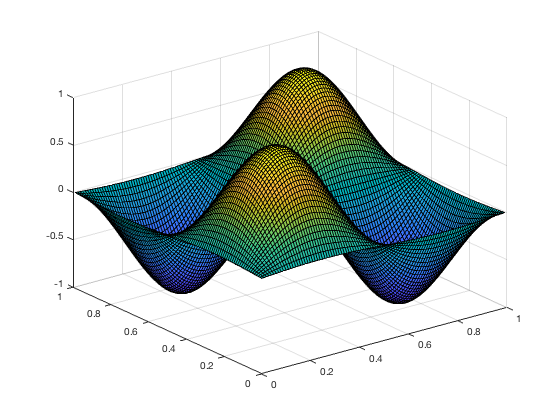
\includegraphics[scale=.5]{Figures/03_01}
        \end{center}

      \item[(d)]
        Do a numerical convergence study in the $L^2$ norm.
        For simplicity, you can just compute the errors based on errors at
        element centers.
        The exact solution is
        \[
          u(x, y) = \sin{2 \pi x} \sin{2 \pi y}
        \]

        I found the order of convergence to be 3, as shown in the following table.
        \begin{center}
          \begin{tabular}{rlll}
            \toprule
              M & h & $L^2$ error & order \\
            \midrule
                7 &   0.14 & 0.002       & - \\
               13 &   0.07 & 0.00037     & 3.04 \\
               25 &   0.04 & 0.000052    & 3.01 \\
              101 & 0.0099 & 0.00000078  & 3.002 \\
              401 & 0.0025 & 0.000000012 & 3.0004 \\
            \bottomrule
          \end{tabular}
        \end{center}

    \end{enumerate}
\end{enumerate}
\end{document}
